% ==========================================================================
% EscutAI: pitch comercial do ecossistema de atendimento do TJPA
% Compilar: pdflatex EscutAI_Ecossistema_Pitch.tex (duas vezes)
%
% Imagens a baixar (Freepik, Pixabay ou Pexels) e salvar em img/. Enquanto faltar
% o arquivo, o slide mostra uma caixa com o nome esperado:
%   img/pessoa_conversando_whatsapp_celular.png
%   img/atendente_balcao_virtual_videochamada.png
%   img/atendimento_presencial_forum_tribunal.png
% ==========================================================================
\documentclass[aspectratio=169,10pt]{beamer}

\usepackage[utf8]{inputenc}
\usepackage[T1]{fontenc}
\usepackage[brazil]{babel}
\usepackage[scaled=0.95]{helvet}
\renewcommand{\familydefault}{\sfdefault}
\usepackage{microtype}
\usepackage{graphicx}
\usepackage{booktabs}
\usepackage{tabularx}
\usepackage{array}
\usepackage{fontawesome5}
\usepackage{tikz}
\usetikzlibrary{arrows.meta,positioning,calc}
\usepackage{hyperref}
\hypersetup{colorlinks=true,urlcolor=petroleo,linkcolor=petroleo}
\graphicspath{{../TJPA/img/}{img/}}

% --------------------------------------------------------------- identidade visual
\definecolor{escuro}{HTML}{053F35}
\definecolor{petroleo}{HTML}{0B5345}
\definecolor{verde}{HTML}{00A884}
\definecolor{menta}{HTML}{16E0A9}
\definecolor{areia}{HTML}{FDE3A7}
\definecolor{nevoa}{HTML}{E8F4F0}
\definecolor{tinta}{HTML}{0E2F33}
\definecolor{cinza}{HTML}{5E6B6B}
\definecolor{ouro}{HTML}{B97A00}
\definecolor{trilho}{HTML}{DDE7E3}
\definecolor{seta}{HTML}{A8D5C6}
\definecolor{rosa}{HTML}{B03060}

\setbeamercolor{normal text}{fg=tinta,bg=white}
\setbeamercolor{structure}{fg=petroleo}
\setbeamercolor{frametitle}{fg=tinta}
\setbeamerfont{frametitle}{size=\Large,series=\bfseries}
\setbeamertemplate{navigation symbols}{}
\setbeamersize{text margin left=0.6cm,text margin right=0.6cm}
\setbeamertemplate{itemize item}{\footnotesize\raise0.1ex\hbox{\textcolor{verde}{\faCaretRight}}}
\setbeamertemplate{frametitle}{%
  \vskip0.2cm
  \begin{minipage}[c]{0.8\paperwidth}\usebeamerfont{frametitle}\usebeamercolor[fg]{frametitle}\insertframetitle\end{minipage}%
  \hfill
  \begin{minipage}[c]{0.12\paperwidth}\raggedleft
    
\includegraphics[height=0.5cm]{logo_escutai_verde.png}\hspace{0.08cm}{\bfseries\small\textcolor{tinta}{Escut}\textcolor{verde}{AI}}%
  \end{minipage}\par
  \vskip-0.12cm
}
\setbeamertemplate{footline}{%
  \leavevmode\hbox to\paperwidth{%
    \hspace{0.6cm}{\tiny\textcolor{cinza}{EscutAI \textperiodcentered\ Ecossistema de atendimento do TJPA}}\hfill
    {\tiny\textcolor{cinza}{\insertframenumber}}\hspace{0.6cm}}\vskip0.18cm}
\AtBeginDocument{\hyphenpenalty=10000 \exhyphenpenalty=10000}

% --------------------------------------------------------------- comandos de apoio
\newcommand{\fundoescuro}{%
  \setbeamercolor{background canvas}{bg=escuro}%
  \setbeamercolor{normal text}{fg=white}%
  \setbeamertemplate{footline}{}%
  \usebeamercolor[fg]{normal text}}
\newcommand{\fonte}[1]{\par\vskip3pt{\tiny\textcolor{cinza}{#1}}}
\newcolumntype{L}{>{\raggedright\arraybackslash}X}
\newcolumntype{P}[1]{>{\raggedright\arraybackslash}p{#1}}

% Imagem externa em img/. #1 arquivo, #2 largura, #3 altura, #4 o que buscar.
% Sem o arquivo, desenha uma caixa com o nome esperado.
\newcommand{\imagem}[4]{%
  \IfFileExists{img/#1}{\includegraphics[width=#2,height=#3,keepaspectratio]{img/#1}}{%
    \begin{tikzpicture}
      \node[draw=cinza,dashed,fill=nevoa,rounded corners=4pt,minimum width=#2,minimum height=#3,
            text width=#2-0.4cm,align=center,text=tinta,font=\tiny]
        {\faImage\\[2pt]\textbf{\detokenize{img/#1}}\\[2pt]#4};
    \end{tikzpicture}}}

% Júlia em círculo branco, para o fundo escuro
\newcommand{\juliacapa}{%
  \begin{tikzpicture}[remember picture,overlay]
    \coordinate (jc) at ($(current page.east)+(-3.1,0)$);
    \fill[white] (jc) circle (2.35);
    \begin{scope}
      \clip (jc) circle (2.3);
      \node at (jc) {
\includegraphics[width=4.1cm]{julia_mascote.png}};
    \end{scope}
  \end{tikzpicture}}

\tikzset{
  % caixas do esquema
  bloco/.style={rounded corners=6pt,align=center,inner sep=4pt,text=tinta,font=\scriptsize},
  blocoar/.style={bloco,fill=nevoa},
  blocoprox/.style={bloco,fill=areia,draw=ouro,line width=1pt},
  % setas
  setaar/.style={-{Stealth[length=6pt]},line width=1.5pt,color=verde},
  setaprox/.style={-{Stealth[length=6pt]},line width=1.5pt,color=ouro,dashed},
  setaduplaprox/.style={{Stealth[length=6pt]}-{Stealth[length=6pt]},line width=1.5pt,color=ouro,dashed},
  % número da etapa e rótulo de seta
  passoar/.style={circle,fill=verde,text=white,inner sep=0,minimum size=.44cm,font=\scriptsize\bfseries},
  passoprox/.style={circle,fill=ouro,text=white,inner sep=0,minimum size=.44cm,font=\scriptsize\bfseries},
  rotulo/.style={font=\fontsize{6.4}{7.4}\selectfont,inner sep=1.5pt,align=center,text=tinta},
  % fluxos em linha
  etapa/.style={rounded corners=4pt,align=center,font=\scriptsize,inner sep=3pt,text=tinta,minimum width=1.85cm,minimum height=.9cm,anchor=west},
  etapahoje/.style={etapa,fill=trilho},
  etapanova/.style={etapa,fill=areia,draw=ouro,line width=1pt,font=\scriptsize\bfseries},
  etapaigual/.style={etapa,fill=nevoa},
}

\title{Um protocolo, todos os canais}
\author{Equipe EscutAI}
\date{Piloto TJPA}

\begin{document}

% ======================================================= 1. capa
{\fundoescuro
\begin{frame}[plain]
  \juliacapa
  \vspace{0.9cm}
  {\color{menta}\bfseries\small ESCUTAI \textperiodcentered\ PROPOSTA PARA O TJPA}\\[0.3cm]
  {\fontsize{30}{34}\selectfont\bfseries Um protocolo,\\o caso inteiro}\\[0.45cm]
  \parbox{8.9cm}{\raggedright\large Com o TKT, o Balcão Virtual e o atendimento presencial já começam sabendo o caso}
\end{frame}}

% ======================================================= 2. oportunidade
\begin{frame}{Quase metade dos pedidos fica sem atendimento}
\centering
\begin{tikzpicture}[x=1cm,y=1cm]
  \foreach \vx/\vv/\vt/\vd/\vc in {
    0/{1.747.124}/Solicitações de atendimento/{Média de agosto e setembro}/verde,
    5.0/{55\%}/Atendimentos realizados/{962.259 atendidos}/petroleo,
    10.0/{784.865}/Pedidos sem atendimento/{Diferença entre os dois números}/ouro}{
    \fill[nevoa,rounded corners=6pt] (\vx,2.75) rectangle ++(4.75,2.75);
    \fill[\vc,rounded corners=2pt] (\vx,2.95) rectangle ++(.09,2.35);
    \node[anchor=west,text=tinta,font=\fontsize{25}{27}\selectfont\bfseries,inner sep=0] at (\vx+.3,4.5) {\vv};
    \node[anchor=west,text=tinta,font=\small\bfseries,inner sep=0] at (\vx+.3,3.6) {\vt};
    \node[anchor=west,text=cinza,font=\scriptsize,inner sep=0] at (\vx+.3,3.15) {\vd};
  }
  \fill[escuro,rounded corners=6pt] (0,.55) rectangle (14.75,2.4);
  \node[text=menta,font=\Large] at (.75,1.47) {\faBullseye};
  \node[anchor=west,text=white,text width=12.8cm,font=\large,align=left,inner sep=0] at (1.4,1.47)
    {\textbf{A oportunidade:} cada ponto percentual a mais de atendimento equivale a cerca de \textbf{17,5 mil pedidos} a mais no mesmo período.};
\end{tikzpicture}
\fonte{Fonte: indicadores do TJPA levantados pela equipe. 1\% de 1.747.124 = 17.471 pedidos (conta direta, não é previsão de resultado).}
\end{frame}

% ======================================================= 3. problema
\begin{frame}{A causa: cada canal guarda o caso em um lugar diferente}
\centering
\vskip3pt
\begin{tikzpicture}[x=1cm,y=1cm]
  \foreach \vx/\vi/\vn/\vh/\vc in {
    0/\faDesktop/Balcão Virtual/{Sala de vídeo,\\sem registro da conversa}/ouro,
    3.75/\faWhatsapp/WhatsApp local/{Celular da unidade,\\fora de qualquer sistema}/verde,
    7.5/\faEnvelope/E-mail/{Caixa de cada\\unidade}/petroleo,
    11.25/\faUniversity/Presencial/{Na memória de\\quem atendeu}/escuro}{
    \fill[nevoa,rounded corners=6pt] (\vx,2.15) rectangle ++(3.5,3.1);
    \fill[\vc,rounded corners=4pt] (\vx+1.3,4.0) rectangle ++(.9,.9);
    \node[text=white,font=\Large] at (\vx+1.75,4.45) {\vi};
    \node[text=tinta,font=\small\bfseries] at (\vx+1.75,3.6) {\vn};
    \node[text=cinza,font=\scriptsize,align=center,text width=3.1cm] at (\vx+1.75,2.85) {\vh};
  }
  \fill[areia,rounded corners=5pt] (0,.45) rectangle (14.75,1.8);
  \node[text=tinta,font=\normalsize,align=center,text width=14cm] at (7.375,1.125)
    {\textbf{A pessoa repete o caso a cada contato, e o servidor começa do zero.}\\[2pt]
     No Balcão Virtual, canal oficial, são \textbf{7 etapas até a resposta}, e o caso é contado de novo.};
\end{tikzpicture}
\fonte{Fonte: mapeamento de jornadas da equipe EscutAI. Etapas contadas no fluxo, não em medição de tempo.}
\end{frame}

% ======================================================= 4. ESQUEMA
\begin{frame}{A solução: o TKT leva o histórico a quem atende}
\centering
\begin{tikzpicture}[x=1cm,y=1cm]
  % --- elementos centrais
  \node[bloco,fill=verde,text=white,minimum width=1.75cm,minimum height=1.6cm,font=\scriptsize\bfseries] (pessoa) at (.875,5.55)
    {\Large\faUser\\[3pt]Pessoa\\atendida};
  \node[blocoar,minimum width=2.75cm,minimum height=1.6cm] (julia) at (4.2,5.55)
    {\normalsize\textcolor{petroleo}{\faWhatsapp}\ \textbf{Júlia}\\[2pt]Responde e faz a triagem\\no WhatsApp};
  \node[bloco,fill=escuro,text=white,minimum width=2.6cm,minimum height=1.6cm] (tkt) at (7.65,5.55)
    {\normalsize\textcolor{menta}{\faHashtag}\ \textbf{TKT}\\[2pt]Protocolo que\\a pessoa guarda};

  % base de histórico
  \fill[escuro,rounded corners=7pt] (.0,2.3) rectangle (8.25,4.05);
  \node[anchor=west,text=white,font=\small\bfseries,inner sep=0] at (.2,3.72) {\textcolor{menta}{\faDatabase}\ Base de histórico};
  \node[anchor=east,text=seta,font=\scriptsize,inner sep=0] at (8.05,3.72) {N atendimentos ligados ao mesmo caso};
  \foreach \vi/\vt in {0/Atendimento 1,1/Atendimento 2,2/Atendimento 3,3/Atendimento N}{
    \pgfmathsetmacro{\x}{.2+\vi*2.03}
    \node[rounded corners=3pt,fill=petroleo,text=white,minimum width=1.75cm,minimum height=.72cm,anchor=west,font=\fontsize{6.4}{7.4}\selectfont,align=center,inner sep=1pt] (a\vi) at (\x,2.82) {\textbf{\vt}\\com TKT};
  }
  \foreach \va/\vb in {0/1,1/2,2/3}{\draw[-{Stealth[length=4pt]},line width=1pt,color=menta] (a\va.east) -- (a\vb.west);}

  % atendimento humano
  \fill[nevoa,rounded corners=7pt] (10.95,2.3) rectangle (14.8,6.35);
  \node[text=tinta,font=\small\bfseries] at (12.875,6.05) {Atendimento humano};
  \node[blocoprox,minimum width=3.45cm,minimum height=1.35cm] (balcao) at (12.875,5.0)
    {\small\faDesktop\ \textbf{Balcão Virtual}\\[2pt]Canal oficial do TJPA};
  \node[blocoprox,minimum width=3.45cm,minimum height=1.35cm] (presencial) at (12.875,3.2)
    {\small\faUniversity\ \textbf{Presencial}\\[2pt]Atendimento na unidade};

  % busca
  \node[blocoprox,minimum width=1.45cm,minimum height=1.5cm,font=\fontsize{6.6}{7.6}\selectfont] (busca) at (9.55,3.2)
    {\normalsize\faSearch\\[2pt]\textbf{Busca}\\\textbf{por TKT}};

  % --- fluxo
  \draw[setaar] (pessoa.east) -- (julia.west);
  \node[passoar] at ($(pessoa.east)!.5!(julia.west)+(0,.33)$) {1};
  \draw[setaar] (julia.east) -- (tkt.west);
  \node[passoar] at ($(julia.east)!.5!(tkt.west)+(0,.33)$) {2};
  \draw[setaar] (julia.south) -- (julia.south |- 0,4.05);
  \node[passoar] at ($(julia.south)+(-.32,-.17)$) {3};
  \node[rotulo,anchor=west] at ($(julia.south)+(.08,-.17)$) {grava cada atendimento};

  \draw[setaprox] (tkt.east) -- (10.95,5.55);
  \node[passoprox] at (9.9,5.88) {4};
  \node[rotulo,text width=1.9cm,anchor=north] at (9.9,5.47) {a pessoa\\informa o TKT};

  \draw[setaprox] (10.95,3.2) -- (busca.east);
  \node[passoprox] at (10.62,3.58) {5};
  \draw[setaduplaprox] (busca.west) -- (8.27,3.2);
  \node[passoprox] at (8.55,3.58) {6};
  \node[rotulo,anchor=north,text width=3.6cm] at (9.55,2.28) {\textbf{5} o atendente busca o TKT\\\textbf{6} a base abre o histórico};

  % --- dashboard e governança
  \node[blocoprox,minimum width=8.25cm,minimum height=.72cm,anchor=west] (painel) at (0,1.28)
    {\small\faChartBar\ \ \textbf{Dashboard web:}\ tempo e resolução para a gestão};
  \draw[setaprox] (4.125,2.28) -- (painel.north -| 4.125,0);
  \node[bloco,fill=trilho,minimum width=5.3cm,minimum height=.72cm,anchor=east,font=\fontsize{6.6}{7.6}\selectfont] at (14.8,1.28)
    {\faLock\ Casos da Ouvidoria não aparecem a outros times.\\O atendente confere a pessoa antes de usar o histórico.};

  % --- resultado e legenda
  \fill[petroleo,rounded corners=4pt] (0,.36) rectangle (14.8,.8);
  \node[text=white,font=\small\bfseries] at (7.4,.58) {\faClock\ Menos tempo de atendimento \qquad \faCheckCircle\ Mais demandas resolvidas};
  \draw[setaar] (.03,.13) -- ++(.7,0);
  \node[anchor=west,font=\tiny,text=tinta,inner sep=2pt] at (.74,.13) {No ar no piloto};
  \draw[setaprox] (2.7,.13) -- ++(.7,0);
  \node[anchor=west,font=\tiny,text=tinta,inner sep=2pt] at (3.41,.13) {Próximo passo da proposta};
\end{tikzpicture}
\end{frame}

% ======================================================= 5. três momentos
\begin{frame}{O mesmo TKT serve em todo atendimento}
\centering
\vskip2pt
\begin{tabular}{@{}c@{\hspace{.35cm}}c@{\hspace{.35cm}}c@{}}
\imagem{pessoa_conversando_whatsapp_celular.png}{4.65cm}{2.75cm}{Pessoa usando o WhatsApp no celular} &
\imagem{atendente_balcao_virtual_videochamada.png}{4.65cm}{2.75cm}{Servidora em videochamada de atendimento} &
\imagem{atendimento_presencial_forum_tribunal.png}{4.65cm}{2.75cm}{Pessoa em atendimento no balcão de um fórum} \\[5pt]
\parbox[t]{4.65cm}{\raggedright\small\textbf{\textcolor{verde}{\faWhatsapp}\ 1. Gera no WhatsApp}\\[3pt]\footnotesize A Júlia atende e gera o TKT. Cada novo atendimento se soma ao histórico.} &
\parbox[t]{4.65cm}{\raggedright\small\textbf{\textcolor{ouro}{\faDesktop}\ 2. Usa no Balcão Virtual}\\[3pt]\footnotesize A pessoa informa o TKT na sala, e o atendente busca o histórico na base.} &
\parbox[t]{4.65cm}{\raggedright\small\textbf{\textcolor{ouro}{\faUniversity}\ 3. Usa no presencial}\\[3pt]\footnotesize Na unidade, a pessoa fornece o TKT, e o atendimento já parte do caso.}
\end{tabular}
\end{frame}

% ======================================================= 6. BALCÃO
\begin{frame}{No Balcão Virtual, o TKT evita a repetição}
\centering
\begin{tikzpicture}[x=1cm,y=1cm]
  \node[anchor=west,font=\small\bfseries,text=cinza,inner sep=0] at (0,6.3) {Hoje};
  \foreach \vi/\vt in {0/{Acessa site\\e sistema},1/{Solicita\\atendimento},2/{Aguarda\\fila virtual},3/{Entra na\\sala virtual},4/{Informa\\os dados},5/{Servidor\\consulta},6/{Recebe a\\resposta}}{
    \pgfmathsetmacro{\x}{\vi*2.13}
    \node[etapahoje] (h\vi) at (\x,5.6) {\vt};
  }
  \foreach \va/\vb in {0/1,1/2,2/3,3/4,4/5,5/6}{\draw[-{Stealth[length=3pt]},line width=.7pt,color=cinza] (h\va.east) -- (h\vb.west);}

  \node[anchor=west,font=\small\bfseries,text=tinta,inner sep=0] at (0,4.72) {Com o TKT: mesmas etapas, duas ficam mais curtas};
  \foreach \vi/\vt/\ve in {0/{Acessa site\\e sistema}/etapaigual,1/{Solicita\\atendimento}/etapaigual,2/{Aguarda\\fila virtual}/etapaigual,3/{Entra na\\sala virtual}/etapaigual,4/{Informa\\o TKT}/etapanova,5/{Abre o\\histórico}/etapanova,6/{Recebe a\\resposta}/etapaigual}{
    \pgfmathsetmacro{\x}{\vi*2.13}
    \node[\ve] (m\vi) at (\x,4.02) {\vt};
  }
  \foreach \va/\vb in {0/1,1/2,2/3,3/4,4/5,5/6}{\draw[-{Stealth[length=3pt]},line width=.9pt,color=petroleo] (m\va.east) -- (m\vb.west);}
  \draw[-{Stealth[length=5pt]},line width=1.2pt,color=verde,rounded corners=5pt] (0,3.2) -- (14.7,3.2);
  \node[fill=white,text=verde,font=\scriptsize\bfseries,inner sep=3pt] at (7.35,3.2) {Dúvida simples: a Júlia responde no WhatsApp, sem fila};

  \foreach \vx/\vc/\vi/\vt/\vd in {
    0/nevoa/\faPhoneSlash/Se a chamada cair/{A pessoa volta com o mesmo TKT, e o caso continua de onde parou.},
    4.95/nevoa/\faCheckCircle/Já existe no piloto/{TKT, histórico por contato, retomada e nota para quem atende no Chatwoot.},
    9.9/areia/\faFlag/Falta construir/{A tela de busca por TKT para o Balcão e o presencial. Depende do TJPA.}}{
    \fill[\vc,rounded corners=5pt] (\vx,1.0) rectangle ++(4.85,1.75);
    \node[anchor=west,text=tinta,font=\footnotesize\bfseries,inner sep=0] at (\vx+.2,2.38) {\vi\ \vt};
    \node[anchor=north west,text=tinta,font=\scriptsize,text width=4.45cm,align=left,inner sep=0] at (\vx+.2,2.05) {\vd};
  }
\end{tikzpicture}
\end{frame}

% ======================================================= 7. PROVA
\begin{frame}{Não é só ideia: o núcleo já funciona no WhatsApp}
\begin{columns}[c,totalwidth=\linewidth]
\begin{column}{0.47\linewidth}
  \centering
  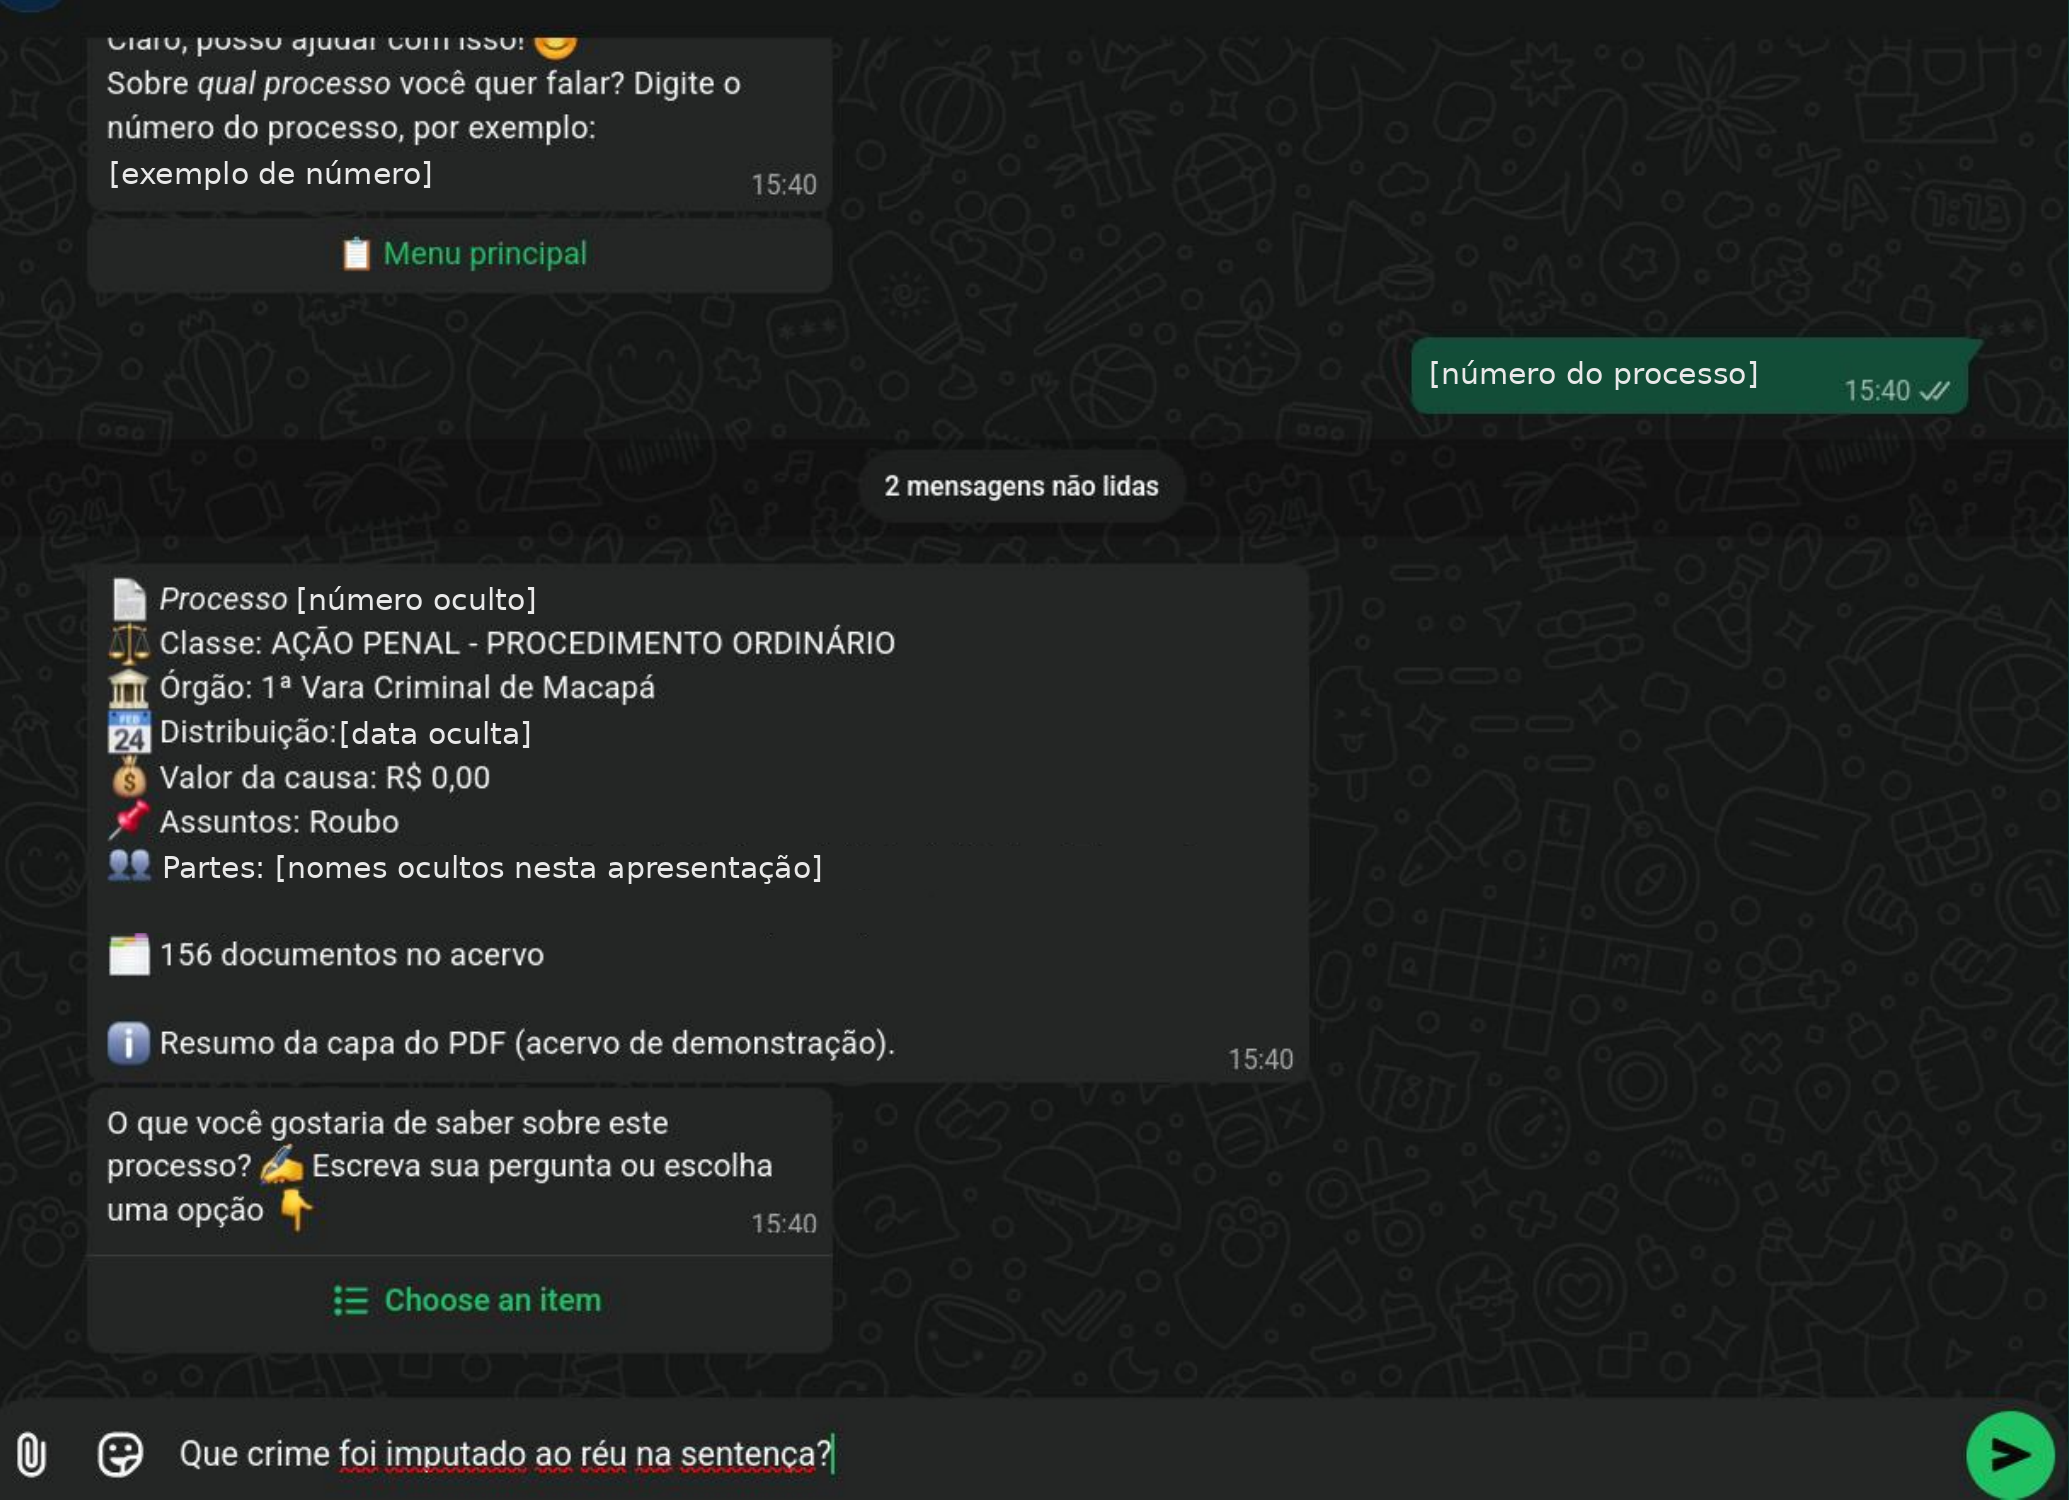
\includegraphics[width=\linewidth,height=5.6cm,keepaspectratio]{whatsapp_demo_anonimizado.png}\\[2pt]
  {\tiny\textcolor{cinza}{Conversa real do piloto, com acervo de demonstração. Nomes, número e data ocultados.}}
\end{column}
\begin{column}{0.5\linewidth}
  \textbf{\textcolor{petroleo}{Entregue e implantado na VM do projeto}}
  \begin{itemize}\footnotesize\setlength\itemsep{1pt}
    \item Júlia no WhatsApp, ligada ao Chatwoot
    \item Protocolo TKT, retomada e histórico
    \item Nota e rascunho de IA para a equipe
    \item Ouvidoria da Mulher, com caso restrito
  \end{itemize}
  \vskip5pt
  \textbf{\textcolor{petroleo}{Testes internos, em acervo de demonstração}}\\[3pt]
  \footnotesize
  \begin{tabularx}{\linewidth}{@{}L r@{}}
    \toprule
    Respostas aprovadas & 40 de 42 \\
    Respostas com fonte citada & 100\% \\
    Tempo típico de resposta & cerca de 2 s \\
    \bottomrule
  \end{tabularx}
  \vskip5pt
  {\scriptsize\textcolor{cinza}{Mostram que a engenharia funciona, com perguntas de teste. O ganho no atendimento real é o que o piloto vai medir.}}
\end{column}
\end{columns}
\end{frame}

% ======================================================= 8. VIABILIDADE
\begin{frame}{Viabilidade: técnica e esforço}
\centering
\begin{tikzpicture}[x=1cm,y=1cm]
  \tikzset{selo/.style={rounded corners=3pt,text=white,font=\fontsize{7}{8}\selectfont\bfseries,inner sep=3pt,anchor=west},
           item/.style={anchor=north west,text=tinta,font=\footnotesize,text width=6.75cm,align=left,inner sep=0},
           aviso/.style={anchor=north west,fill=areia,rounded corners=4pt,text=tinta,font=\footnotesize,text width=6.7cm,align=left,inner sep=4pt}}
  % ---------- técnica
  \fill[nevoa,rounded corners=6pt] (0,-.2) rectangle (7.25,6.35);
  \node[text=petroleo,font=\Large] at (.45,5.9) {\faServer};
  \node[anchor=west,text=tinta,font=\normalsize\bfseries,inner sep=0] at (.85,5.9) {Técnica};
  \node[selo,fill=verde] at (.3,5.3) {VIÁVEL: JÁ ESTÁ NO AR};
  \node[item] (t1) at (.3,4.95) {\textbf{Roda na VM do projeto} (1 vCPU, 3,9 GB), sem serviço extra: banco SQLite e modelo de busca local.};
  \node[item] (t2) at ($(t1.south west)+(0,-7pt)$) {\textbf{Resposta em 1,8 a 2,0 s} (mediana) e até 3,7 s (p95), em teste com a IA real e 42 perguntas.};
  \node[item] (t3) at ($(t2.south west)+(0,-7pt)$) {\textbf{Peças prontas:} TKT, histórico e nota ao atendente. \textbf{Falta} a tela de busca por TKT.};
  \node[aviso] at ($(t3.south west)+(0,-10pt)$) {\faExclamationTriangle\ \textbf{Folga curta:} o backend usa 724 de 900 MiB (80\%). Antes de expandir, rever a memória.};

  % ---------- esforço
  \fill[nevoa,rounded corners=6pt] (7.5,-.2) rectangle (14.75,6.35);
  \node[text=petroleo,font=\Large] at (7.95,5.9) {\faTools};
  \node[anchor=west,text=tinta,font=\normalsize\bfseries,inner sep=0] at (8.35,5.9) {Esforço};
  \node[selo,fill=ouro] at (7.8,5.3) {MÉDIO: DEPENDE DO TJPA};
  \node[item] (f1) at (7.8,4.95) {\textbf{Já construído:} 7,5 mil linhas de código e 537 testes automáticos.};
  \node[item] (f2) at ($(f1.south west)+(0,-7pt)$) {\textbf{O que falta} (tamanho estimado pela equipe):};
  \foreach \vi/\vt/\vz/\vc in {1/{Campo de serviço}/P/verde,2/{Busca por TKT com perfis}/P/verde,3/{Dashboard web (2 páginas)}/M/ouro,4/{Entrada no Balcão}/TJPA/rosa}{
    \node[anchor=north west,text=tinta,font=\footnotesize,inner sep=0,text width=4.5cm] at ($(f2.south west)+(0,-.16-\vi*.46+.46)$) {\vt};
    \node[fill=\vc,text=white,rounded corners=2pt,font=\fontsize{7}{8}\selectfont\bfseries,minimum width=.85cm,inner sep=2pt,anchor=east] at ($(f2.south west)+(6.7,-.34-\vi*.46+.46)$) {\vz};
  }
  \node[aviso] at ($(f2.south west)+(0,-2.2)$) {\faClock\ \textbf{O caminho longo é a decisão do TJPA:} quem acessa, como conferir a pessoa e o prazo de guarda (DPO).};

  \node[anchor=north west,text=cinza,font=\fontsize{5.8}{6.8}\selectfont,text width=14.7cm,align=left,inner sep=0] at (0,-.3)
    {P = pequeno, M = médio; sem prazo em dias, que só dá para fixar depois da decisão do TJPA. Memória: medição na VM em 6/nov/2026. Tempos: \texttt{docs/AVALIACAO.md}. Os custos de operação estão no slide seguinte.};
\end{tikzpicture}
\end{frame}

% ======================================================= 9. CUSTO
\begin{frame}{Custo de operar: pesa o WhatsApp, não a IA}
\centering
\begin{tikzpicture}[x=1cm,y=1cm]
  \tikzset{cartao/.style={fill=nevoa,rounded corners=6pt},
           num/.style={anchor=west,text=tinta,font=\fontsize{15}{16}\selectfont\bfseries,inner sep=0},
           rot/.style={anchor=west,text=cinza,font=\fontsize{6.8}{8}\selectfont,inner sep=0,text width=4.3cm,align=left}}
  \node[anchor=west,text=tinta,font=\footnotesize\bfseries,inner sep=0] at (0,3.05) {Custo por 1.000 atendimentos};
  % IA
  \fill[nevoa,rounded corners=6pt] (0,.0) rectangle (4.75,2.85);
  \node[text=petroleo,font=\normalsize] at (.35,2.5) {\faRobot};
  \node[anchor=west,text=tinta,font=\small\bfseries,inner sep=0] at (.65,2.5) {IA (Sabiazinho-4)};
  \node[num] at (.25,1.8) {cerca de R\$ 8};
  \node[rot,anchor=north west] at (.25,1.4) {1,4 perguntas livres por atendimento e cerca de R\$ 0,0057 por resposta. Menus e botões não chamam a IA.};
  % WhatsApp
  \fill[areia,rounded corners=6pt] (4.9,.0) rectangle (9.85,2.85);
  \node[text=petroleo,font=\normalsize] at (5.25,2.5) {\faWhatsapp};
  \node[anchor=west,text=tinta,font=\small\bfseries,inner sep=0] at (5.55,2.5) {WhatsApp (Meta)};
  \node[num] at (5.15,1.8) {cerca de R\$ 370};
  \node[rot,anchor=north west] at (5.15,1.4) {10,5 mensagens da Júlia por atendimento, a R\$ 0,035 por mensagem (hipótese, a confirmar na tabela da Meta).};
  % infra
  \fill[nevoa,rounded corners=6pt] (10.0,.0) rectangle (14.75,2.85);
  \node[text=petroleo,font=\normalsize] at (10.35,2.5) {\faServer};
  \node[anchor=west,text=tinta,font=\small\bfseries,inner sep=0] at (10.65,2.5) {Infraestrutura e licenças};
  \node[num] at (10.25,1.8) {R\$ 0 adicional};
  \node[rot,anchor=north west] at (10.25,1.4) {A VM, o Chatwoot e a busca já existem e não têm licença por uso. O custo mensal da VM não foi levantado.};
\end{tikzpicture}
\vskip4pt
\footnotesize
\begin{tabularx}{\linewidth}{@{}>{\raggedright\arraybackslash}p{3.2cm} *{4}{>{\raggedleft\arraybackslash}X}@{}}
\toprule
\textbf{Atendimentos} & \shortstack[r]{\textbf{IA}\\\textbf{por mês}} & \shortstack[r]{\textbf{WhatsApp}\\\textbf{por mês}} & \shortstack[r]{\textbf{Total}\\\textbf{por mês}} & \shortstack[r]{\textbf{Total}\\\textbf{por ano}} \\
\midrule
1.000 por mês & R\$ 8 & R\$ 330 & R\$ 340 & R\$ 4.100 \\
10.000 por mês & R\$ 80 & R\$ 3.640 & R\$ 3.720 & R\$ 44.600 \\
100.000 por mês & R\$ 800 & R\$ 36.720 & R\$ 37.510 & R\$ 450.200 \\
\bottomrule
\end{tabularx}
\par\vskip2pt\raggedright{\tiny\textcolor{cinza}{Valores arredondados, sem imposto, câmbio nem faixas de desconto por volume. Premissas medidas na VM em 6/nov/2026: 1,4 respostas da IA por atendimento (37 protocolos de uso interno do piloto) e 10,5 mensagens enviadas por atendimento (4 conversas reais de WhatsApp, amostra pequena). Custo da resposta: estimativa a partir do teto de contexto. Preços: \href{https://www.maritaca.ai/en/pricing}{Maritaca}. Tarifa da Meta de R\$ 0,035 por mensagem: hipótese a partir de fontes secundárias, a confirmar na \href{https://developers.facebook.com/documentation/business-messaging/whatsapp/pricing}{tabela da Meta}; as 1.000 mensagens gratuitas por número ao mês já estão descontadas.}}
\end{frame}

% ======================================================= 10. VALOR
\begin{frame}{Onde se ganha tempo e resolução, e como provar}
\vskip2pt
\footnotesize
\begin{tabularx}{\linewidth}{@{}P{2.6cm}LLP{3.6cm}@{}}
\toprule
\textbf{Momento} & \textbf{O que muda} & \textbf{Ganho esperado} & \textbf{Prova no dashboard} \\
\midrule
Antes da fila & A Júlia resolve a dúvida simples & Fila menor no Balcão & Resolvidos só pela Júlia \\ \addlinespace[3pt]
Início do atendimento & O atendente busca o TKT e lê o histórico & Menos tempo, sem repetir o caso & Duração e repetição do caso \\ \addlinespace[3pt]
Presencial & O servidor já parte do caso & Menos retrabalho na unidade & Buscas por TKT \\ \addlinespace[3pt]
Retorno & A pessoa volta com o mesmo TKT & O caso continua de onde parou & Resolução no 1º contato \\
\bottomrule
\end{tabularx}
\vskip7pt
\centering
\begin{tikzpicture}[x=1cm,y=1cm]
  \fill[nevoa,rounded corners=5pt] (0,0) rectangle (7.25,2.0);
  \node[anchor=west,text=petroleo,font=\fontsize{22}{24}\selectfont\bfseries,inner sep=0] at (.2,1.15) {+14\%};
  \node[anchor=west,text=tinta,font=\scriptsize,text width=4.5cm,align=left,inner sep=0] at (2.3,1.0)
    {de casos resolvidos por hora entre 5.179 atendentes com assistente de IA (+34\% entre novatos), fora do Judiciário.};
  \node[anchor=west,text=cinza,font=\tiny,inner sep=0] at (.2,.2) {Brynjolfsson, Li e Raymond, NBER 31161, 2023.};
  \fill[areia,rounded corners=5pt] (7.5,0) rectangle (14.75,2.0);
  \node[anchor=west,text=tinta,font=\scriptsize,text width=6.75cm,align=left,inner sep=0] at (7.75,1.0)
    {\textbf{\faBalanceScale\ Nosso compromisso:} não prometer número antes de medir. Ainda não há dados reais de tempo nem de resolução. Medimos a linha de base, comparamos antes e depois e fixamos as metas com o TJPA.};
\end{tikzpicture}
\end{frame}

% ======================================================= 9. CONFIANÇA
\begin{frame}{Por que o Tribunal pode confiar}
\centering
\vskip3pt
\begin{tikzpicture}[x=1cm,y=1cm]
  \foreach \vx/\vy/\vi/\vt/\vd/\vc in {
    0/3.1/\faSearch/Não inventa resposta/{Só responde com fonte aprovada. Sem evidência, admite que não sabe e encaminha.}/verde,
    7.5/3.1/\faUserCheck/O humano decide/{A Júlia organiza e encaminha. O rascunho de IA é rotulado e o servidor revisa.}/petroleo,
    0/.75/\faLock/TKT não basta sozinho/{O TKT nunca devolve o caso à pessoa. O histórico só aparece ao atendente, que confere a identidade antes de usar.}/ouro,
    7.5/.75/\faHeart/Casos sensíveis à parte/{Na Ouvidoria da Mulher, o caso não aparece a outros times nem vai para a IA.}/rosa}{
    \fill[nevoa,rounded corners=6pt] (\vx,\vy) rectangle ++(7.25,2.1);
    \fill[\vc,rounded corners=4pt] (\vx+.25,\vy+.65) rectangle ++(.8,.8);
    \node[text=white,font=\normalsize] at (\vx+.65,\vy+1.05) {\vi};
    \node[anchor=west,text=tinta,font=\small\bfseries,inner sep=0] at (\vx+1.3,\vy+1.6) {\vt};
    \node[anchor=north west,text=tinta,font=\footnotesize,text width=5.65cm,align=left,inner sep=0] at (\vx+1.3,\vy+1.3) {\vd};
  }
\end{tikzpicture}
\par\vskip5pt{\scriptsize\textcolor{cinza}{Em aberto com o TJPA: enquadramento na Res. CNJ 615/2025 com a área de IA e prazo de guarda do histórico com a DPO (90 dias no piloto). O piloto não declara conformidade.}}
\end{frame}

% ======================================================= 10. CAMINHO
\begin{frame}{Começar pequeno, medir e expandir}
\centering
\begin{tikzpicture}[x=1cm,y=1cm]
  \foreach \vx/\vn/\vt/\vd/\vc in {
    0/1/Medir/{Dashboard web e linha de base de 30 dias}/petroleo,
    3.75/2/Busca por TKT/{Tela do atendente, com perfis de acesso}/ouro,
    7.5/3/Usar na unidade/{Balcão Virtual e presencial em 1 ou 2 unidades}/ouro,
    11.25/4/Comparar/{Antes e depois, para decidir a expansão às 299 unidades}/verde}{
    \fill[nevoa,rounded corners=5pt] (\vx,3.0) rectangle ++(3.5,2.6);
    \node[fill=\vc,text=white,circle,inner sep=0,minimum size=.62cm,font=\small\bfseries] at (\vx+.45,5.1) {\vn};
    \node[anchor=west,text=tinta,font=\small\bfseries,text width=2.55cm,align=left,inner sep=0] at (\vx+.85,5.1) {\vt};
    \node[anchor=north west,text=tinta,font=\footnotesize,text width=3.05cm,align=left,inner sep=0] at (\vx+.22,4.5) {\vd};
  }
  \foreach \vx in {3.52,7.27,11.02}{\draw[-{Stealth[length=4pt]},line width=1pt,color=petroleo] (\vx,4.3) -- ++(.21,0);}
  \fill[areia,rounded corners=5pt] (0,.75) rectangle (14.75,2.7);
  \node[anchor=north west,text=tinta,font=\small\bfseries,inner sep=0] at (.25,2.5) {O que pedimos ao TJPA};
  \node[anchor=north west,text=tinta,font=\footnotesize,text width=6.8cm,align=left,inner sep=0] at (.25,2.0)
    {\faCaretRight\ Autorizar a busca por TKT no Balcão e no presencial\\[4pt]
     \faCaretRight\ Definir quem vê o histórico e como conferir a pessoa};
  \node[anchor=north west,text=tinta,font=\footnotesize,text width=6.8cm,align=left,inner sep=0] at (7.5,2.0)
    {\faCaretRight\ Indicar 1 ou 2 unidades para o piloto\\[4pt]
     \faCaretRight\ Pactuar as metas de tempo e de resolução};
\end{tikzpicture}
\end{frame}

% ======================================================= 11. ROADMAP PÓS-PITCH
\begin{frame}{Se vencermos: 5 etapas, cada uma com prova}
\centering
\vskip3pt
\begin{tikzpicture}[x=1cm,y=1cm]
  \tikzset{rotlin/.style={anchor=west,text=cinza,font=\fontsize{6.6}{7.6}\selectfont\bfseries,inner sep=0,text width=1.1cm,align=left},
           entrega/.style={text=tinta,font=\footnotesize\bfseries,text width=2.5cm,align=center,inner sep=0},
           prova/.style={text=tinta,font=\scriptsize,text width=2.46cm,align=center,inner sep=0},
           decisao/.style={text=tinta,font=\scriptsize\bfseries,text width=2.3cm,align=center,inner sep=0}}
  % rótulos das linhas
  \node[rotlin] at (0,3.75) {ENTREGA};
  \node[rotlin] at (0,1.85) {PROVA};
  \node[rotlin] at (0,.42) {DECISÃO};
  \foreach \vi/\vn/\vt/\vp/\vc/\vic/\ve/\vv/\vd in {
    0/1/Mobilizar/Início/ouro/\faFileSignature/{Termo e regra de acesso}/{Termo assinado e regra aprovada pela DPO}/{Regra aprovada?},
    1/2/Construir/Meses 1 a 2/petroleo/\faSearch/{TKT integrado ao Balcão Virtual}/{Demonstração no canal oficial e linha de base}/{Integrou? Metas fixadas?},
    2/3/Testar/Meses 3 a 5/petroleo/\faUniversity/{Teste no Balcão\\e dashboard\\gerencial}/{Amostra com atendentes e métricas no dashboard}/{Atendentes validam?},
    3/4/Avaliar/Meses 6 a 7/verde/\faChartBar/{Antes e depois, contra as metas}/{Relatório entregue ao TJPA}/{Expandir ou ajustar?},
    4/5/Expandir/Mês 8 em diante/verde/\faSitemap/{Todas as unidades,\\com operação\\e suporte}/{Mesmos indicadores por unidade}/{Indicadores se mantêm?}}{
    \pgfmathsetmacro{\vx}{1.15+\vi*2.72}
    % seta da etapa
    \fill[\vc] (\vx,5.0) -- ++(2.5,0) -- ++(.2,.42) -- ++(-.2,.42) -- ++(-2.5,0) -- ++(.2,-.42) -- cycle;
    \node[anchor=center,text=white,font=\footnotesize\bfseries,inner sep=0] at (\vx+1.35,5.57) {\vn. \vt};
    \node[anchor=center,text=white,font=\fontsize{7}{8}\selectfont,inner sep=0] at (\vx+1.35,5.24) {\vp};
    % entrega
    \fill[nevoa,rounded corners=5pt] (\vx,2.72) rectangle ++(2.6,2.13);
    \node[text=\vc,font=\Large] at (\vx+1.3,4.4) {\vic};
    \node[entrega] at (\vx+1.3,3.4) {\ve};
    % prova
    \draw[seta,line width=.7pt,rounded corners=5pt] (\vx,1.12) rectangle ++(2.6,1.46);
    \node[prova] at (\vx+1.3,1.85) {\vv};
    % decisão
    \fill[areia,rounded corners=5pt] (\vx,0) rectangle ++(2.6,.98);
    \node[decisao] at (\vx+1.3,.49) {\vd};
  }
\end{tikzpicture}
\par\vskip4pt\raggedright{\tiny\textcolor{cinza}{A etapa seguinte só começa com a decisão anterior, tomada pelo TJPA. Metas fixadas antes do teste. Prazos: proposta de partida, a fechar com o TJPA.}}
\end{frame}

% ======================================================= 12. fecho
{\fundoescuro
\begin{frame}[plain]
  \juliacapa
  \vspace{0.9cm}
  {\color{menta}\bfseries\small ESCUTAI \textperiodcentered\ A JUSTIÇA QUE ESCUTA VOCÊ}\\[0.3cm]
  {\fontsize{26}{31}\selectfont\bfseries Contar uma vez.\\Resolver mais rápido.}\\[0.45cm]
  \parbox{8.9cm}{\raggedright\large O TKT e o histórico já funcionam no WhatsApp. O próximo passo é abrir esse histórico a quem atende no Balcão Virtual e no presencial.}
\end{frame}}

\end{document}
